\documentclass{beamer}
\usepackage[utf8]{inputenc}
\usepackage{graphicx, epsfig}
\usepackage{amsmath,mathrsfs,amsfonts,amssymb}
\usepackage{subfig}
\usepackage{floatflt}
\usepackage{epic,ecltree}
\usepackage{mathtext}
\usepackage{fancybox}
\usepackage{fancyhdr}
\usepackage{multirow}
\usepackage{enumerate}
\usepackage{epstopdf}
\usepackage{multicol}
\usepackage{algorithm}
\usepackage[noend]{algorithmic}
\def\algorithmicrequire{\textbf{Input:}}
\def\algorithmicensure{\textbf{Output:}}
\usetheme{Copenhagen}%{Singapore}%{Warsaw}%{Warsaw}%{Darmstadt}
\usecolortheme{whale}
%\definecolor{beamer@blendedblue}{RGB}{15,120,80}
%----------------------------------------------------------------------------------------------------------
\title[\hbox to 56mm{Matrix Completion  \hfill\insertframenumber\,/\,\inserttotalframenumber}]
{Low-Rank Matrix Completion Project}
\author[ROY team]{\\
				{\small \textbf{Authors:} Artem Bochkarev, Roman Isachenko \\
					Ilya Zharikov, Anne-Laure Ducrocq}}
\institute[SkolTech]{Skolkovo Institute of Science and Technology \\
	Numerical Linear Algebra course 
    \vspace{0.3cm}
}
\date{December 16, 2016.}
%--------------------------------------------------------------------------------
\begin{document}
%--------------------------------------------------------------------------------
\begin{frame}
%\thispagestyle{empty}
\titlepage
\end{frame}
%--------------------------------------------------------------------------------
\begin{frame}{Problem Statement}
\begin{block}{Task}	
	Given the amount of observed matrix entries to reconstruct low-rank matrix approximation.
\end{block}
\vspace{0.3cm}
\textbf{Applications:}
\begin{itemize}
	\item  recommender systems;
	\item image-processing;
	\item imputation of NAs for genomic data;
	\item rank estimation for SVD.
\end{itemize}
\end{frame}
%--------------------------------------------------------------------------------
\begin{frame}{Problem Statement}
\textbf{Notations:}
\begin{itemize}
	\item $M$~--- $n \times m$ unknown matrix;
	\item $\Omega \in \{1, \dots, n\} \times \{1, \dots, m\}$ indices of observed elements;
	\item 
	$$
	P_{\Omega} (M) = 
	\begin{cases}
	M_{ij}, &\text{if} \, (i, j) \in \Omega;\\
	0, &\text{otherwise}.
	\end{cases}
	$$
\end{itemize}
\begin{block}{Optimization Task ($NP$-hard)}
	\vspace{-0.5cm}
	\begin{align*}
		\mathop{\text{minimize}}\limits_{X \in \mathbb{R}^{n \times m}} \quad & 
		\text{rank} (X) \\
		\text{subject to} \quad & P_{\Omega} (X) = P_{\Omega} (M)
	\end{align*}
\end{block}

\end{frame}

%--------------------------------------------------------------------------------
\begin{frame}{Relaxations}
	\begin{block}{Original Task ($NP$-hard)}
		\vspace{-0.2cm}
		\begin{align*}
		\mathop{\text{minimize}}\limits_{X \in \mathbb{R}^{n \times m}} \quad 
		\text{rank} (X), \quad 
		\text{subject to} \quad P_{\Omega} (X) = P_{\Omega} (M)
		\end{align*}
	\end{block}
	\vspace{0.3cm}
	\footnotesize
	\begin{columns}[c]
	\column{0.5\textwidth}
	\begin{block}{SVP}
		\vspace{-0.3cm}
		\begin{align*}
		\mathop{\text{minimize}}\limits_{X \in \mathbb{R}^{n \times m}} \quad & 
		\| P_{\Omega} (X) - P_{\Omega} (M) \|_F^2 \\
		\text{subject to} \quad & \text{rank} (X) \leq k
		\end{align*}
	\end{block}
	
	\begin{block}{RISMF}
		\vspace{-0.3cm}
		\begin{align*}
		\mathop{\text{minimize}}\limits_{\substack{	U \in \mathbb{R}^{n \times k} \\ V \in \mathbb{R}^{k \times m}}} \quad & \| U \|^2_F + \| V \|^2_F \\
		\text{subject to} \quad &  P_{\Omega} (UV) = P_{\Omega} (M) 
		\end{align*}
	\end{block}
	\column{0.5\textwidth}	
	\begin{block}{SVT}
		\vspace{-0.3cm}
		\begin{align*}
		\mathop{\text{minimize}}\limits_{X \in \mathbb{R}^{n \times m}} \quad & \tau \| X \|_* + \| X \|_F^2 \\
		\text{subject to} \quad & P_{\Omega} (X) = P_{\Omega} (M)
		\end{align*}
	\end{block}
	\begin{block}{SoftImpute}
		\vspace{-0.3cm}
		\begin{align*}
		\mathop{\text{minimize}}\limits_{X \in \mathbb{R}^{n \times m}} \quad & 
		\| X \|_* \\
		\text{subject to} \quad & \| P_{\Omega} (X) - P_{\Omega} (M) \|_F \leq \delta
		\end{align*}
	\end{block}
\end{columns}
	
\end{frame}
%--------------------------------------------------------------------------------
\begin{frame}{Related Works}
\begin{enumerate}
	\item Candes E. J., Recht B. Exact matrix completion via convex optimization. 2009.
	\item Cai J. F., Candes E. J., Shen Z. A singular value thresholding algorithm for matrix completion. 2010.
	\item Mazumder R., Hastie T., Tibshirani R. Spectral regularization algorithms for learning large incomplete matrices. 2010.
	\item Jain P., Meka R., Dhillon I. S. Guaranteed rank minimization via singular value projection. 2010.
	\item Takacs G. et al. Scalable collaborative filtering approaches for large recommender systems. 2009.
	\item Vandereycken B. Low-rank matrix completion by Riemannian optimization. 2013.
\end{enumerate}
\end{frame}
%--------------------------------------------------------------------------------
\begin{frame}{SVP (Jain P., Meka R., Dhillon I. S., 2010)}

	\begin{block}{Relaxation}
		\vspace{-0.5cm}
		\begin{align*}
		\mathop{\text{minimize}}\limits_{X \in \mathbb{R}^{n \times m}} \quad 
		\| P_{\Omega} (X) - P_{\Omega} (M) \|_F^2, \quad
		\text{subject to} \quad \text{rank} (X) \leq k
		\end{align*}
	\end{block}
\vspace{0.3cm}
\begin{algorithmic}[1] 
	\REQUIRE $\Omega, P_\Omega(M), k, \eta$; 
	\ENSURE $X$;
	\STATE $X:= 0$;
	\REPEAT
	\STATE $X := X - \eta P_{\Omega}^{-1}\left(P_{\Omega}(X) - P_{\Omega}(M)\right)$;
	\STATE {$U, \Sigma, V := SVD(X)$};
	\STATE $X := U_k \Sigma_k V_k^T$;
	\UNTIL {$\|P_{\Omega}(M) - P_{\Omega}(X)\|_F / \|P_{\Omega}(X)\|_F > \varepsilon$}
\end{algorithmic}
\end{frame}
%--------------------------------------------------------------------------------
\begin{frame}{SVT (Cai J. F., Candes E. J., Shen Z., 2010)}
		\begin{block}{Relaxation}
			\vspace{-0.5cm}
			\begin{align*}
			\mathop{\text{minimize}}\limits_{X \in \mathbb{R}^{n \times m}} \quad \lambda \| X \|_* + \| X \|_F^2, \quad
			\text{subject to} \quad P_{\Omega} (X) = P_{\Omega} (M)
			\end{align*}
		\end{block}
	\vspace{0.3cm}
	\begin{algorithmic}[1]
		\REQUIRE $\Omega, M, \varepsilon, \lambda, \eta$;
		\ENSURE $X$;
		\STATE $Y := \eta P_{\Omega}(M)$;
		\REPEAT
		\STATE $X := S_{\lambda} (Y)$;
		\STATE $P_{\Omega}\left(Y\right) := P_{\Omega}\left(Y\right)+\eta P_\Omega \left(M - X\right)$;
		\UNTIL {$\| P_{\Omega}(X - M)\|_F/\| P_{\Omega}(M) \|_F > \varepsilon$}
	\end{algorithmic}
	\vspace{0.3cm}
$$
S_{\lambda} (W) = U [D - \lambda I]_+ V^*; \quad U, D, V := SVD(W)
$$
\end{frame}
%--------------------------------------------------------------------------------
\begin{frame}{SoftImpute (Hastie T., Tibshirani R., 2010)}
		\begin{block}{Lagrangian Relaxation}
			\vspace{-0.5cm}
			\begin{align*}
			\mathop{\text{minimize}}\limits_{X \in \mathbb{R}^{n \times m}} \quad & 
			\lambda \| X \|_* + \|P_\Omega(X) - P_\Omega(M) \|_F^2
			\end{align*}
		\end{block}

\begin{algorithmic}[1]
	\REQUIRE $M, \Omega, \varepsilon, \lambda_1 > \dots > \lambda_k$;
	\ENSURE sequence $X_{\lambda_1}, \dots, X_{\lambda_k}$;
	\STATE $X := 0$;
	\FOR{$i=1,\dots,k$}
	\REPEAT
	\STATE $X := S_{\lambda_i} (P_\Omega(M) + P_\Omega^\bot (X))$;
	
	\UNTIL{$\|P_{\Omega}(M) - P_{\Omega}(X)\|_F / \|P_\Omega(M)\|_F > \varepsilon$}
	\STATE {$X_{\lambda_i} := X$};
	\ENDFOR
\end{algorithmic}
$$
	P_{\Omega}^\bot (M) = M - P_{\Omega} (M).
$$
\end{frame}
%--------------------------------------------------------------------------------
\begin{frame}{RIMSF}

\begin{block}{Relaxation}
	\vspace{-0.3cm}
	\begin{align*}
	\mathop{\text{minimize}}\limits_{\substack{	U \in \mathbb{R}^{n \times k} \\ V \in \mathbb{R}^{k \times m}}} \quad \|P_{\Omega} (UV) - P_{\Omega} (M)\|_F^2 + \lambda \left(\| U \|^2_F + \| V \|^2_F\right)
	\end{align*}
\end{block}
	
\begin{algorithmic}[1]
	\REQUIRE $M, \Omega, \varepsilon, \lambda, \eta$;
	\ENSURE {$U, V$};
	\STATE {Initialization of $U, V$ with small random numbers};
	\REPEAT
	\FOR {$(i, j) \in \Omega$}
	\STATE {Gradient step for $U[i, :]$ and $V[:, j]$ by regularized error function};
	\ENDFOR
	\UNTIL{$\|P_{\Omega}(M) - P_{\Omega}(UV)\|_F / \|P_\Omega(M)\|_F > \varepsilon$}
\end{algorithmic}
\end{frame}
%--------------------------------------------------------------------------------
\begin{frame}{Numerical Experiments}
\begin{itemize}
	\item Synthetic data
	
	Low-rank matrices with random noise.
	\item Low-rank images
	
	Visual demonstration of algorithms.
	\item Assessment dataset
	
	Real dataset for collaborating filtering.
\end{itemize}

\end{frame}
%--------------------------------------------------------------------------------
\begin{frame}{Synthetic Data}
\begin{figure}[h]
	\centering
	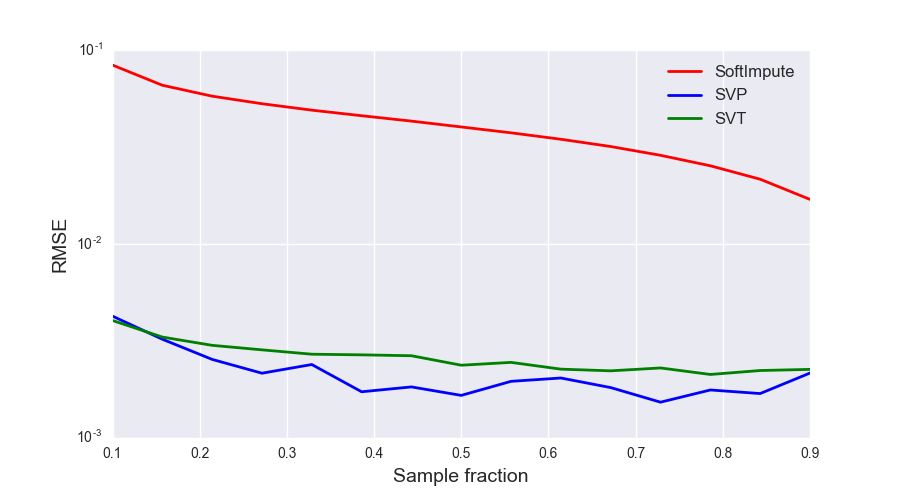
\includegraphics[width=1\linewidth]{./../results/synthetic/exper_1/synthetic_nsamp_rmse.png}
	\label{heat_map}
\end{figure}
\end{frame}
%--------------------------------------------------------------------------------
\begin{frame}{Synthetic Data}
	\begin{figure}[h]
		\centering
		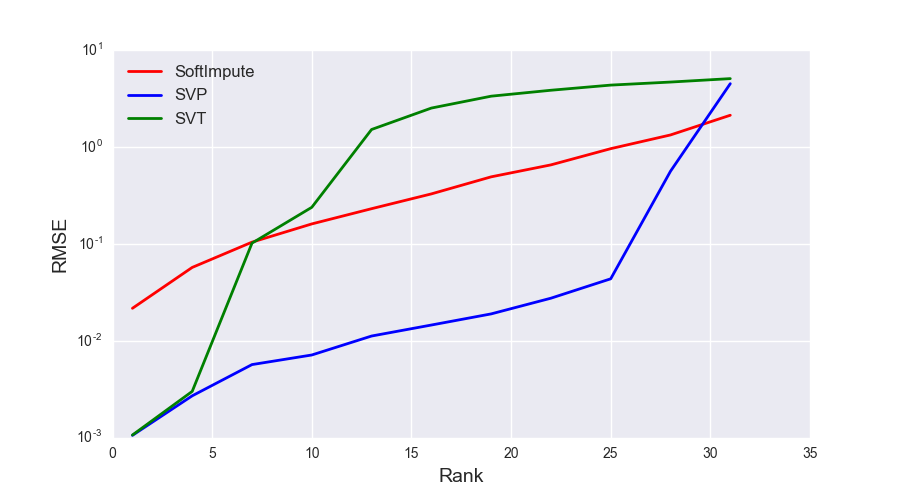
\includegraphics[width=1\linewidth]{./../results/synthetic/exper_2/synthetic_rank_rmse.png}
		\label{heat_map}
	\end{figure}
\end{frame}
%--------------------------------------------------------------------------------
\begin{frame}{Synthetic Data}
	\begin{figure}[h]
		\centering
		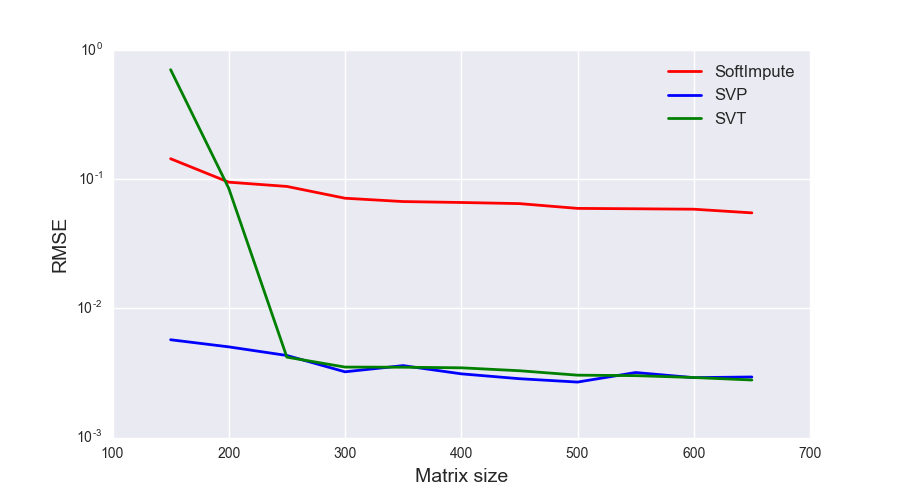
\includegraphics[width=1\linewidth]{./../results/synthetic/exper_3/synthetic_size_rmse.png}
		\label{heat_map}
	\end{figure}
\end{frame}
%--------------------------------------------------------------------------------
\begin{frame}{Images}
\end{frame}
%--------------------------------------------------------------------------------
\begin{frame}{Assessment data}
	
\end{frame}
%--------------------------------------------------------------------------------

\end{document} 